\subsection{БД в парсинге}
Важной составляющей микросервиса является база данных. 
В ней хранится совсем вся информация о пользователях и о структуре манги.
Главной особенностью базы в данном проекте является то, что можно контролировать количество пользователей, которые используют сервис.
Таким образом возможно принимать решение о том нужно ли заниматься оптимизацией или улучшением компонент сервера. 
БД также позволяет легко получить доступ к данным, ограничить его же другим пользователям и легко перенести информацию от одного сервера в другой.

Однако, выше были перечисленные общие преимущества для микросервисов.
Главным же преимуществом базы данных в данном проекте заключается в том, что можно сохранять структуру глав к любой манге.
Таким образом не придется делать большое количество запросов на каждого пользователя. 
Возможно ограничиться только запросами на загрузку картинок с сервера.
При использовании клиентского сервиса в виде мессенджера телеграм, возможно загружать мангу, создавая статьи.
Каждой статье в телеграме предоставляется своя ссылка. 
Так при генерировании статьи пользователем, ссылка может сохраниься в базе данных. 
В случаях, когда какая-то манга является популярной, возможно лишь выдавать в последствии ссылку уже подготовленную статью.
Преимущество статьи выражается в том, что телеграм подготовил весь необходимый удобный интерфейс. Поэтому просмотр комикса выглядит локанично.

Если к API подключить сервис по облачному хранилищу или же прямо непосредственно на сервере хранить все уже загруженные и сгенерированные главы в виде pdf, 
то вполне возможно загружать в БД пути к определенным файлам, чтобы не делать заново генерацию.

БД может помочь в дальнейшем развитии проекта, а именно организации подписки на рассылку выхода новой главы конкретной манги. 
Так можно сделать воркер, способный в фоне раз в какое-то время обновлять структуру глав манги.
При обновлении этой структуры, будет происходить рассылка пользователям, которые подписались на обновление комикса.
Структуру глав манги можно хранить в виде документа JSON.

Особенностью конструирования схемы БД является то, что обновление ее происзводится при помощи миграций \cite{migrations-cite}.

\subsubsection{Описание сущностей БД}
На рисунке~\ref{db-struct-pic} представлена схема БД, которая используется на момент написания ВКР.

\begin{figure}
    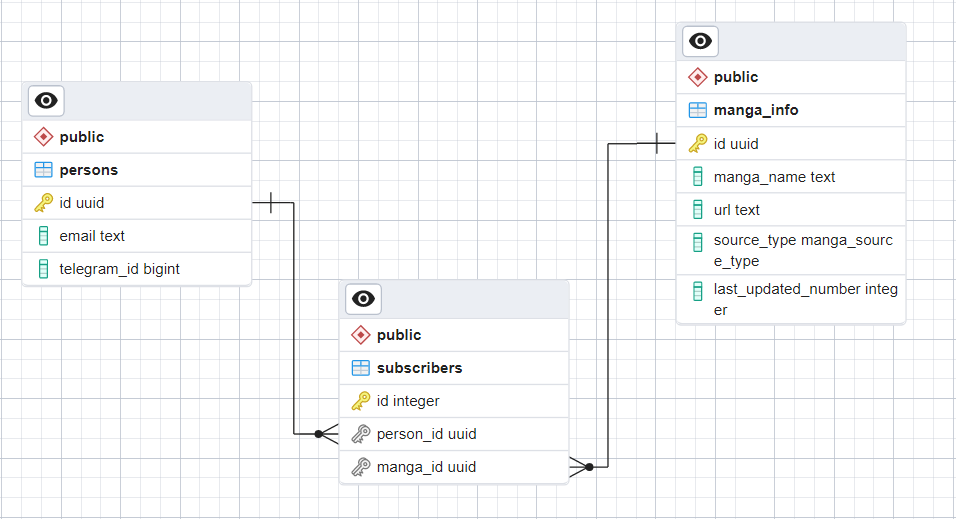
\includegraphics[scale=0.5]{imgs/db-struct}
    \caption{Схема БД проекта}
    \label{db-struct-pic}
\end{figure}

В этой схеме можно увидеть несколько таблиц:
\begin{itemize}
    \item persons,
    \item manga\_info,
    \item subscribers.
\end{itemize}

Опишем предназначение каждой из таблиц.

\paragraph{Persons}
Таблица persons нужна для того, чтобы записывать информацию о пользователе. 
Информация может быть о его логине, ID в каком-то мессенджере или любая другая информация, которая может помочь идентефицировать пользователя.
Также возможно хранить тут контактую информацию, по которой возможно уведомлять о рассылке.
Сейчас эта таблица нужна для того, чтобы сохранить email, на который нужно присылать мангу, чтобы синхронизировать ту с электронной книгой.
Таким образом происходит защита от спам рассылки на другие email. Сначала пользователю обязательно нужно залогиниться в API, подтвердить свой email,
а уже затем возможно отправлять сгенерированные файлы себе.

Регистрация будет происходить таким образом для массового пользователя, что ему необходимо получить код, который будет в файле, отправленный на электронную книгу.
Так возможно добиться подтверждения от пользователя, что почта точно принадлежит нужному человеку.

\paragraph{Manga\_info}
В таблице manga\_info, как понятно из названия, хранится информация о структуре манги.
В этой таблице в дальнейшем можно хранить ссылки на статью, которая сгенерируется для клиентского сервиса в телеграме.
Когда множество пользователей захочет скачать себе одну главу, повторная информация будет браться из этой таблицы, дабы не нагружать сайт запросами лишний раз.
Таблица также имеет идентефикатор типа источника информации. Эта информация нужна для того, чтобы понять какой тип алгоритма расшифровки структуры глав манги нужно применять.
Сделано это было потому, что структура сайтов и, соответственно, организация манги на них может быть совершенно разной. Например, на многих сайтов есть поддержка нескольких языков.
Соответственно базовая структура глав манг изменится, путом добавления строчки языка.

\paragraph{Subscribers}
Таблица subscribers является связующим звеном между таблицей manga\_info и persons. 
Она, как понятно из названия, создана для того, чтобы можно было отслеживать людей, которые подписались на какую-то конерктную мангу.
Так можно делать рассылки сразу нескольким людям, используя в коде лишь один запрос с соединением данных.
Подписка и отписка от рассылки будет происходить совсем просто: достаточно добавить строчку с ID пользователя и желаемой манги.